% !TeX root = ../main.tex
% Add the above to each chapter to make compiling the PDF easier in some editors.

\chapter{Introduction}\label{chapter:introduction}

\section{Connectomics}
To understand the internal workings of brain neuroscientists have been trying to reconstruct its 'neural circuitry' also termed as a connectome, which illustrates how neurons are connected with each other. The first ever brain to be studied at this intricate detail was that of C. Elegans in the 1980's ~\cite{whiteCElegans} with serial section electron microscopy(EM) images and the neurons were traced manually. 

Since then, EM methods have improved many folds, generating petabytes of data, even for a small Fruit Fly brain\textcolor{red}{cite Drosophilia paper}. So, the process of segmenting and tracing neurons have been delegated to Machine Learning(ML) algorithms, with humans pitching in only for error correction or initial training data generation. 

Neuron tracing problem is a hard nut to crack. This can be attributed to its large volume size, multiple image artifacts, numerous closely intertwined segments of vivid shapes etc. \textcolor{red}{show images illustrating problems}. Hence, the results of most algorithms are either not satisfactory or they are too slow and entail complicated postprocessing steps, limiting their scope to only inside a computer science lab far away from being used as a tool directly by neuroscientists.

This work tries to build upon from existing method and approaches which researchers have been working on from deca


\section{Connectomics Pipeline}

%\begin{figure}[htpb]
%  \centering
%  \newcommand{\mywidthSmall}{0.15\textwidth}
%  \newcommand{\mywidth}{0.20\textwidth}
%  \newcommand{\myheight}{0.20\textwidth}
%  \newcolumntype{X}{ >{\centering\arraybackslash} m{\mywidth} }
%  \setlength\tabcolsep{3mm} 
%  \def\arraystretch{0}%  1 is the default
%  \begin{tabular}{XXX}
%    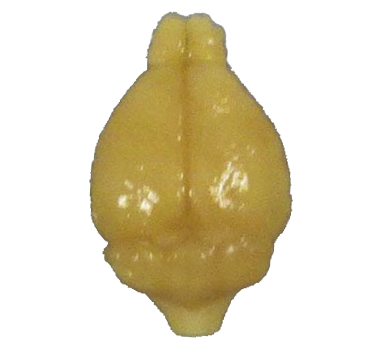
\includegraphics[height=\myheight, width=\mywidthSmall,keepaspectratio]{data/images/brain.png}&
%    \includegraphics[height=\myheight, width=\mywidth,keepaspectratio]{data/images/slicing.jpg}&
%	\includegraphics[height=\myheight, width=\mywidthSmall,keepaspectratio]{data/images/slices.png}\\
%	%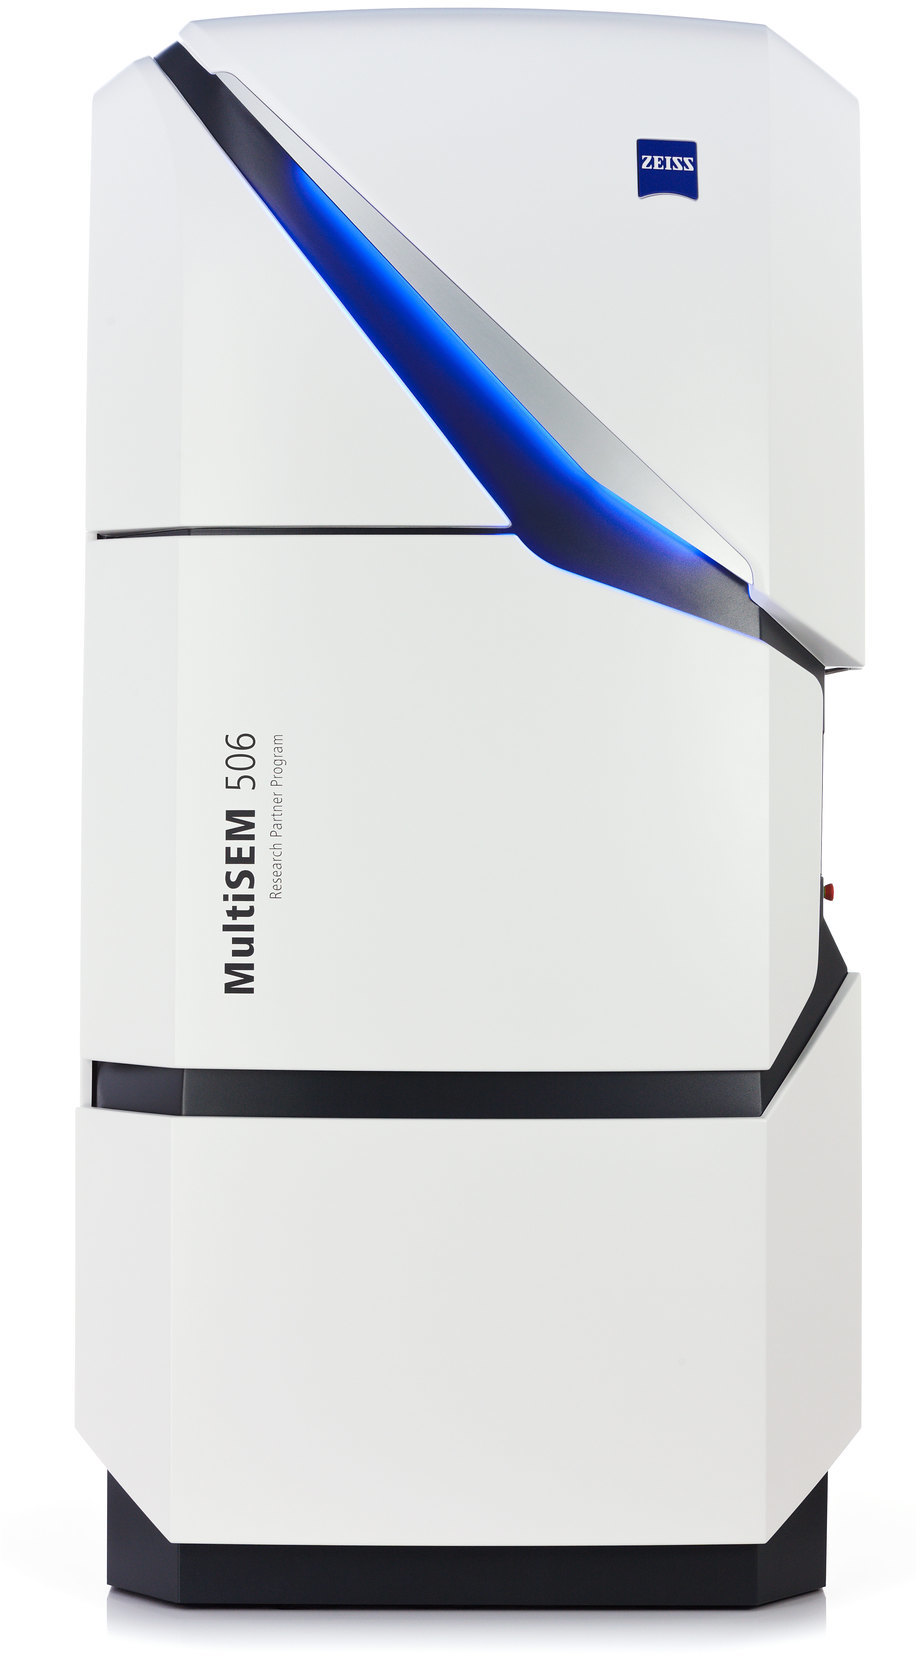
\includegraphics[height=0.1\textheight,width=\mywidth,keepaspectratio]{data/images/emMicroscope.jpg}&
%	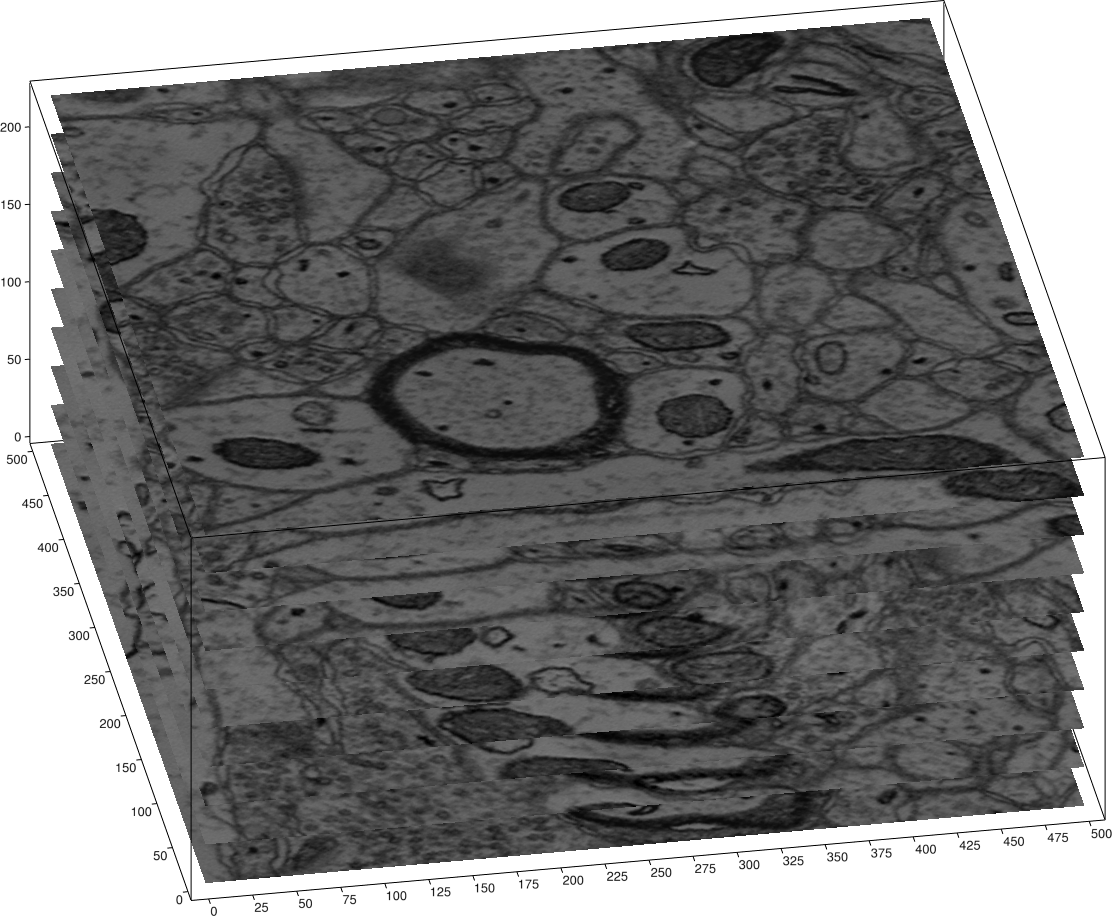
\includegraphics[height=\myheight,width=\mywidth]{data/images/imStack.png}&
%	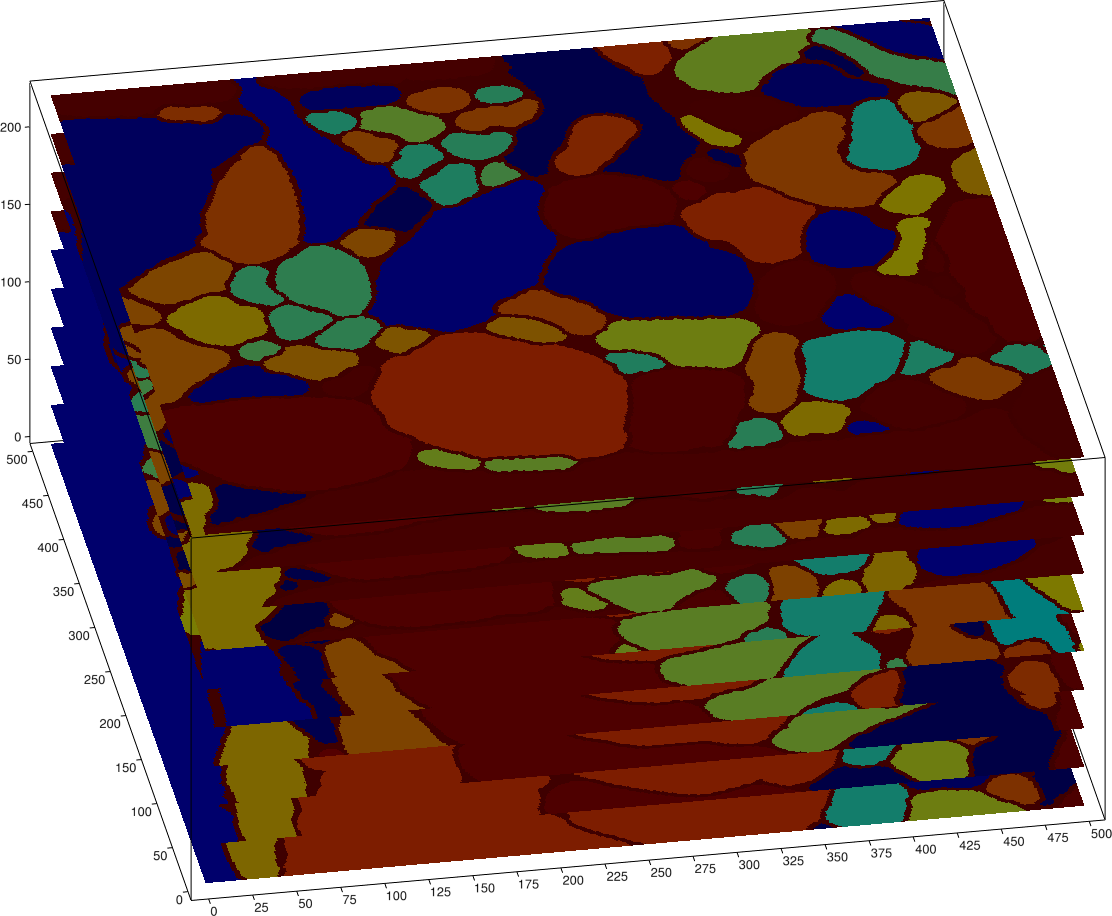
\includegraphics[height=\myheight,width=\mywidth]{data/images/segStack.png}&
%	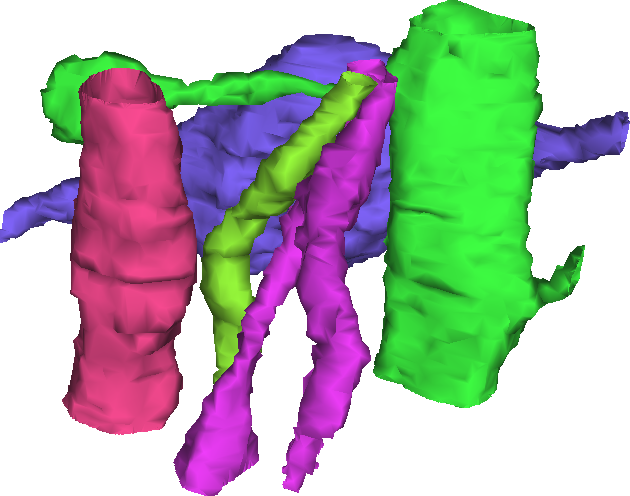
\includegraphics[height=\myheight,width=\mywidth]{data/images/seg3d.png}\\
%  \end{tabular}
%	\caption{Connectomics Pipeline.}
%	\label{fig:connectomicsPipeline}
%\end{figure}

\begin{figure}[htpb]
	\newcommand{\mywidth}{0.44\textwidth}
	\centering
	\begin{subfigure}[b]{\mywidth}
		\centering
		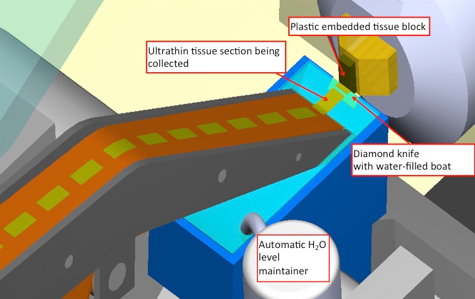
\includegraphics[width=\textwidth]{data/images/slicing/slicing_diagram.png}
		\caption{\label{fig:slicing_diagram}}
	\end{subfigure}
	\hspace{3mm}
	\begin{subfigure}[b]{\mywidth}
		\centering
		\includegraphics[width=\textwidth]{data/images/slicing/slicing.png}
		\caption{\label{fig:slicing}}
	\end{subfigure}
	\hspace{3mm}
	\begin{subfigure}[b]{\mywidth}
		\centering
		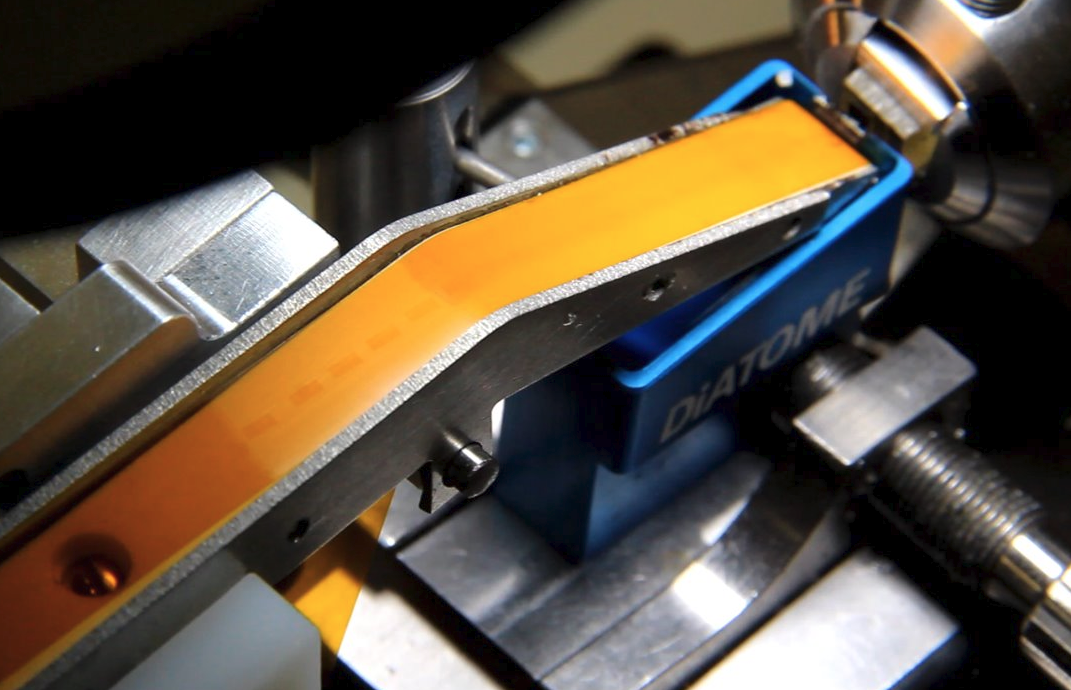
\includegraphics[width=\textwidth]{data/images/slicing/slicing_close.png}
		\caption{\label{fig:slicing_close}}
	\end{subfigure}
	\hspace{3mm}
	\begin{subfigure}[b]{\mywidth}
		\centering
		\includegraphics[width=\textwidth]{data/images/slicing/wafer.png}
		\caption{\label{fig:wafer}}
	\end{subfigure}
	\caption{Automated high-throughput serial sectioning setup. \subref{fig:slicing_diagram} explains a automated serial sectioning setup \cite{Baena2019}, \cite{Hayworth2006}. \subref{fig:slicing} shows a similar setup at Lichtman Lab, Harvard. \subref{fig:slicing_close} shows thin rectangular slices being collected on the conveyor tape. \subref{fig:wafer} shows a set of slices on wafer, later to be imaged using an electron microscope. All images are courtesy of Lichtman Lab \cite{LichtmanLab} and its members.}
	\label{fig:emSlicing}
\end{figure}

\begin{figure}[htpb]
	\newcommand{\mywidth}{0.44\textwidth}
	\newcommand{\mywidthlarge}{0.66\textwidth}
	\centering
	\begin{subfigure}[b]{\mywidth}
		\centering
		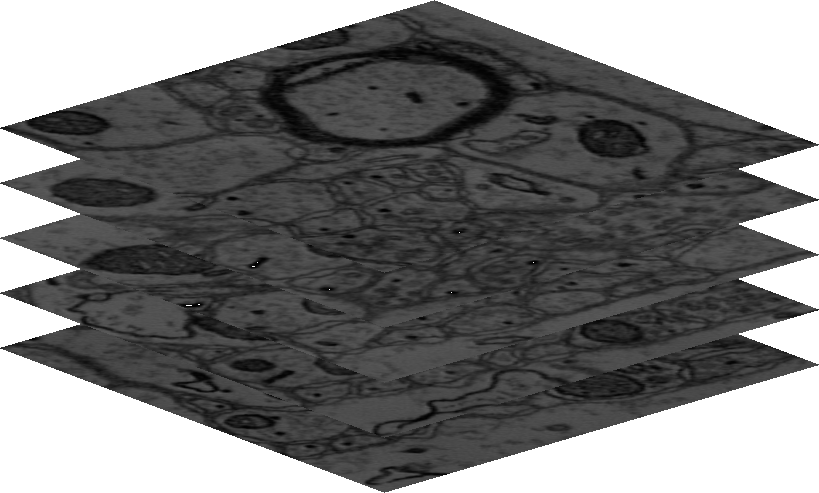
\includegraphics[width=\textwidth]{data/images/stack/im.png}
		\caption{\label{fig:im_stack}}
	\end{subfigure}
	\hspace{3mm}
	\begin{subfigure}[b]{\mywidth}
		\centering
		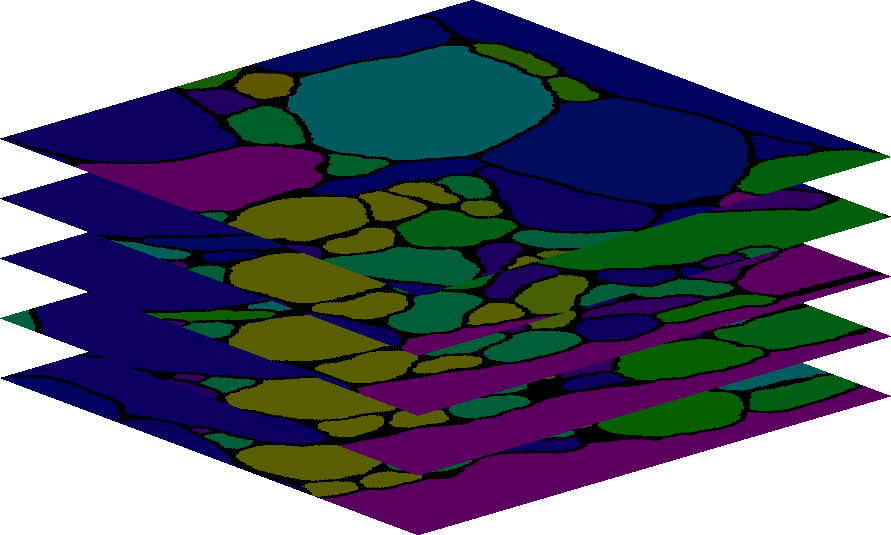
\includegraphics[width=\textwidth]{data/images/stack/seg.png}
		\caption{\label{fig:seg_stack}}
	\end{subfigure}
	\hspace{3mm}
	\begin{subfigure}[b]{\mywidthlarge}
		\centering
		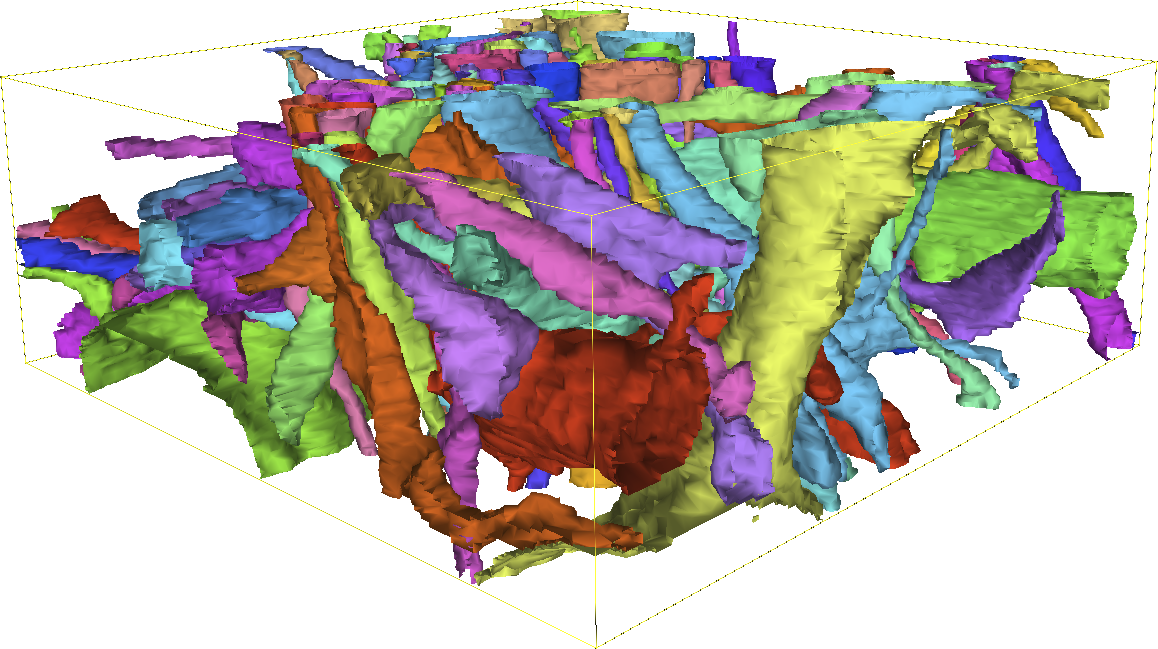
\includegraphics[width=\textwidth]{data/images/stack/seg_3d.png}
		\caption{\label{fig:seg_3d}}
	\end{subfigure}
	\caption{3D EM image stack and segmentation. \subref{fig:im_stack} shows stacking of a few aligned 2D images along $Z$ axis. Alignment can be tough due to image artifacts and deformations during slicing. \subref{fig:seg_stack} shows the corresponding segmentation map created manually. Annotators glance across multiple slices to figure tougher segment boundaries. \subref{fig:seg_3d} shows the final manual segmentation output.}
	\label{fig:emSegmenting}
\end{figure}

The construction of the brain connectomes starts by slicing the brain tissue as thin as possible and imaging the 2D slices using an electron microscope, typically at resolution of $3 - 10$ nanometers. After imaging, the 2D images are stacked, aligned and processed to remove noise and other artifacts.\textcolor{red}{cite alignment papers, ask Adi}. Finally, this 3D image is segmented, often by doing multiple, laborious iterations of automatic segmentation and manual error correction to obtain a connectivity graph of the neuronal processes. Figure \ref{fig:connectomicsPipeline} shows a simplified succinct connectomics pipeline, starting from the brain tissue, alignment and segmentation. After segmentation multiple other analysis can be performed, which would entail more processing.


\section{Quirks of EM Data}
A Electron Microscopy(EM) image stack can contain numerous of segments which are arbitrarily and closely intertwined with each other. The membranes demarcating different cells can be thin and tough to distinguish even by trained humans. \autoref{fig:snemiDataset} shows a EM dataset \textcolor{red}{cite SNEMI} illustrating thin boundaries, closely packed nature of those neuronal segments and intertwined structure of the segments.

Apart from previously mentioned properties, EM datasets especially from serial section EM usually have some more quirks like:
\begin{itemize}
  \item The resolution of the 3D image may not be isotropic. For serial section EM, the in-plane resolution along $X$ and $Y$ axis is usually $2$ to $5$ times higher than the $Z$ resolution which is governed by the slice thickness 
  \item 2D image slices can have large artifacts due to physical folds or knife marks while imaging.
  \item There can be sharp discontinuities across slices due to misalignment, missing slices etc.
  \item The boundaries of segments can break at some points or get blurred and hard to distinguish.
  \item The size in pixels of one volume can be in the order of $10K*10K*5K$ voxels and a single segment can encompass from one diagonal end to the other.
\end{itemize}

Thus, EM datasets are much more complex to segment compared to other natural non medical imaging datasets, and thus specialized algorithms need to be developed to tackle them.


\begin{figure}[htpb]
  \centering
  \newcommand{\mywidth}{0.4\textwidth}
  \newcommand{\myheight}{0.3\textwidth}
  \newcommand{\mywidthLarge}{0.3\textwidth}
  \newcommand{\myheightLarge}{0.3\textwidth}
  \newcolumntype{X}{ >{\centering\arraybackslash} m{\mywidth} }
  \setlength\tabcolsep{3mm} % default value: 6pt
  \def\arraystretch{0}%  1 is the default
  \begin{tabular}{XX}
	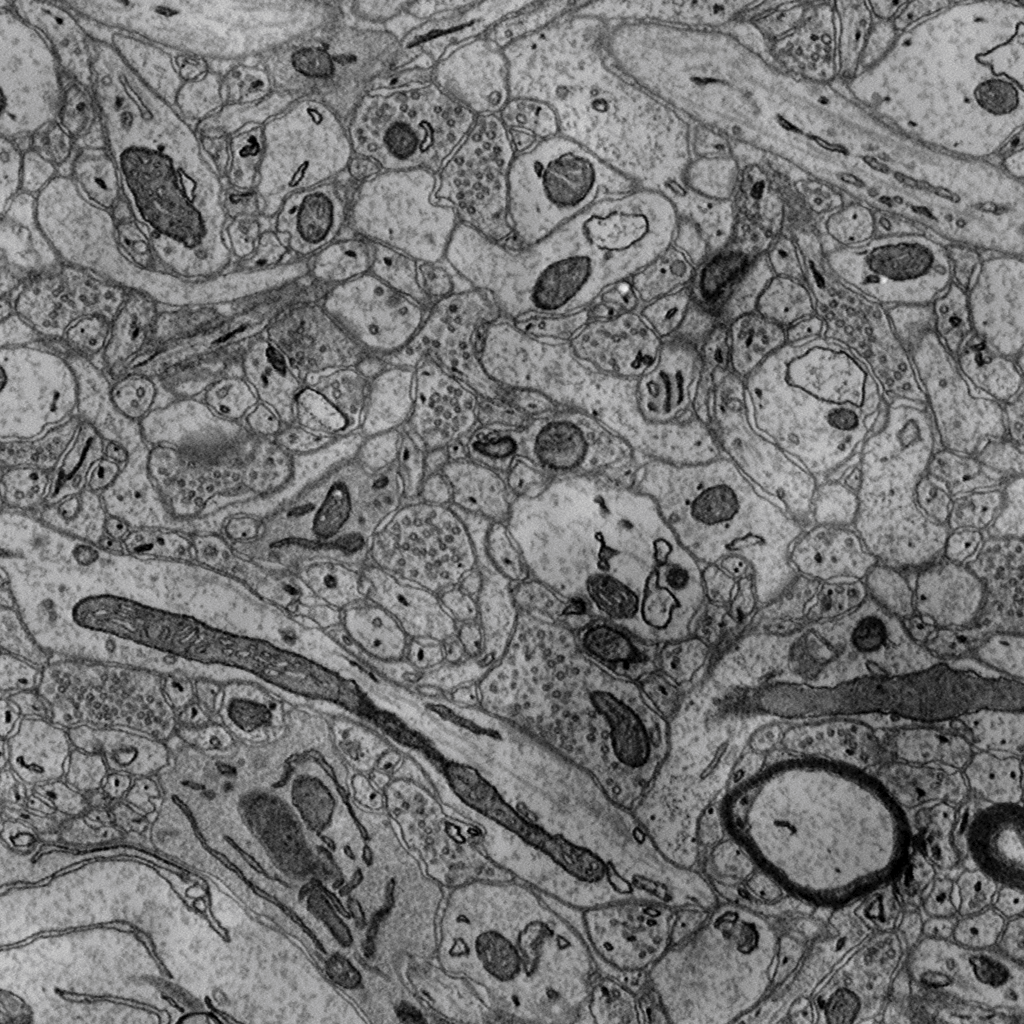
\includegraphics[height=\myheight,width=\mywidth, keepaspectratio]{data/images/snemiGlimpse/snemiTrainSliceImages.png}\caption*{2D image slice.}&
	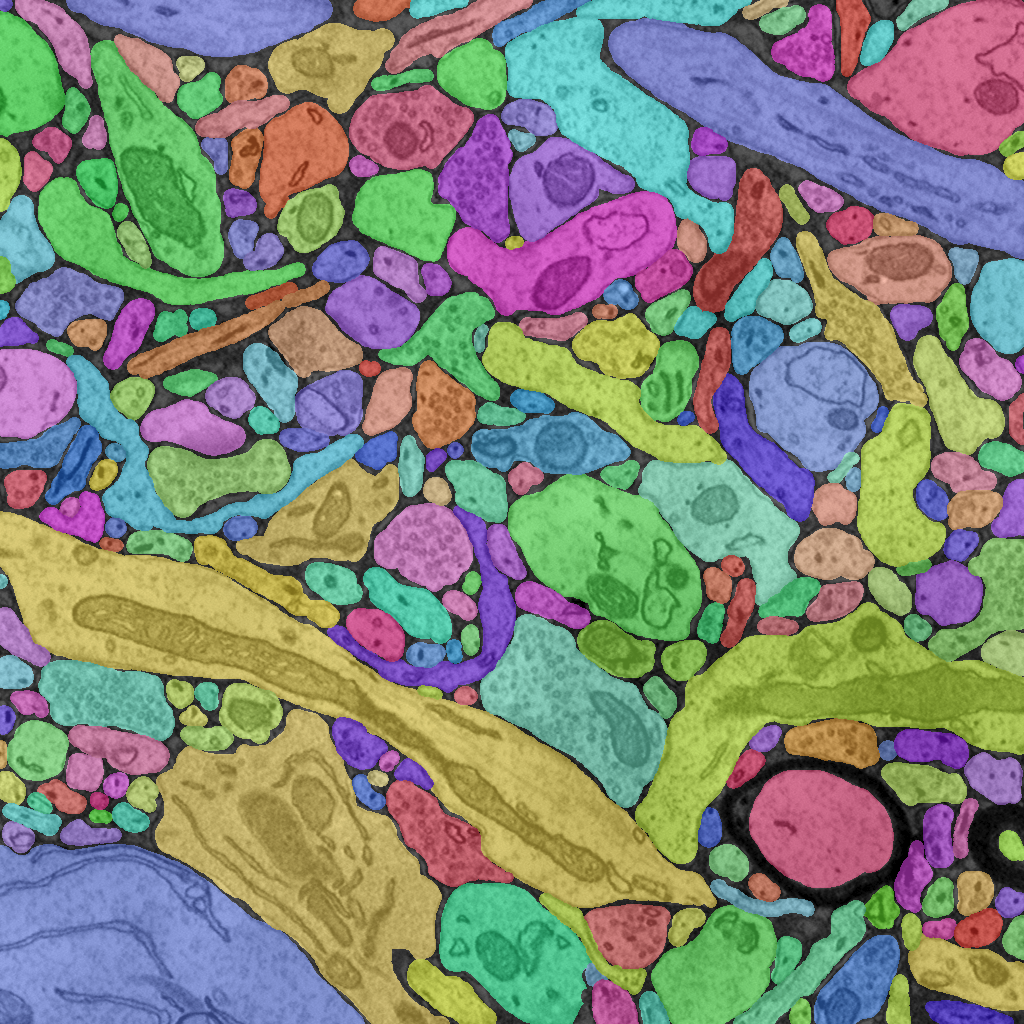
\includegraphics[height=\myheight,width=\mywidth,keepaspectratio]{data/images/snemiGlimpse/snemiTrainSliceLabels.png}\caption*{2D segmentation} \\
	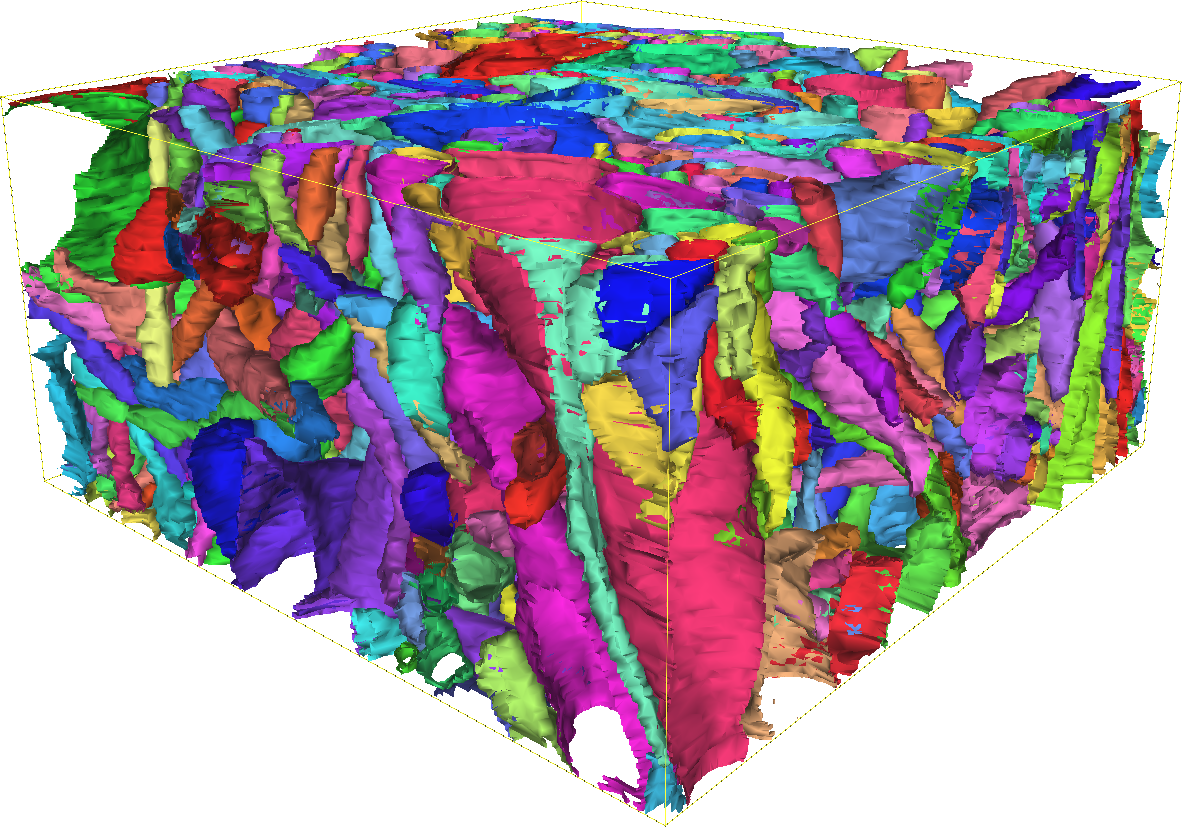
\includegraphics[height=\myheight,width=\mywidth,keepaspectratio]{data/images/snemiGlimpse/snemi3DSeg.png}\caption*{3D segmentation.}&
	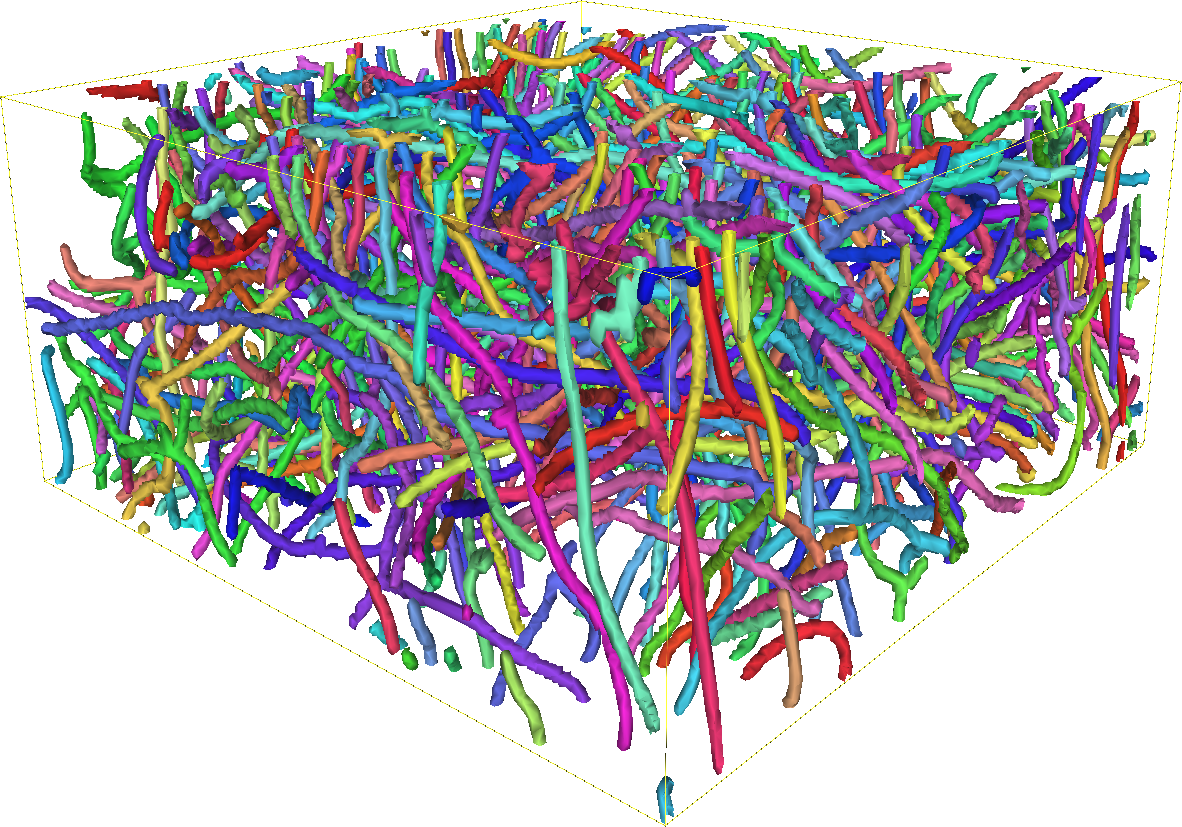
\includegraphics[height=\myheight,width=\mywidth,keepaspectratio]{data/images/snemiGlimpse/snemi3DSkelContext.png}\caption*{3D skeletons.}
  \end{tabular}
	\caption{The SNEMI Dataset (\cite{SNEMI3D}). It was created as part of a Connectomics challenge to advance segmentation methods. The dimensions are relatively small - $100*1024*1024$ voxels with resolution of $30*6*6$ nm. }
	\label{fig:snemiDataset}
\end{figure}


\section{Segmentation Methods}

\subsection{Boundary based Methods}
To segment multiple 3D segments as shown in \autoref{fig:snemiDataset} one of the usual methods is to first perform semantic segmentation into two classes - foreground, which consists of all the internal pixels of segments, and background, which consists of the extracellular space. Given such a perfect semantic mask, it is trivial to obtain the instance segmentation of each cell using simple connected component analysis. One can then match segments from different slices using intersection of union scores. \textcolor{red}{cite boundary matching paper} \textcolor{blue}{ask donglai how boundary mask is segmented?}

Another commonly used approach for EM 3D segmentation is to represent boundaries as affinity graphs, first introduced by \cite{Turaga2010}. In its simplest form affinity graphs are similar to boundary masks - if a voxel and its immediate next neighbor lie in same segment then a high value, usually $1$, is stored at that voxel. In this scenario the affinity graph would be of $3$ channels, one each for the immediate next neighbour along $X$, $Y$ and $Z$. Affinity graphs can be created for distant neighbors also, leading to more channels, and encoding long distance connectivity, useful for thin elongated segments, used by \cite{Kisuk2017}. After obtaining such soft partition graph, the final segmentation can be done using standard graph partitioning methods or even connected components analysis, as shown in \cite{Turaga2010} or 3D affinity based watershed transform, used by \cite{Kisuk2017} and \cite{Aleks2015WatershedClustering}.

A common underlying idea in both methods is that they break down the segmentation problem into two steps. First is a local prediction step, where boundary is predicted based on local image textures and edges. Second is somewhat more global, which looks at connectivity of voxels and performs hierarchical clustering of oversegmented clusters based on shape and connectivity. The dismantling of the segmentation problem helps to tackle multi instance segmentation problem and makes it amenable for Deep Learning (DL) based methods.

A major issue with these pipeline processes is that a minute leak in the boundary segmentation can lead to false merge. To somewhat avoid such false merges, the hyper-parameters of watershed clustering are tuned so as to keep the results optimally over-segmented. This is done keeping in mind that its easier to correct false splits for humans rather than fixing false merges. Nevertheless, manually agglomerating over-segmentation is still laborious and not extendable to larger volumes.
Second issue, encountered in DL based boundary prediction methods with a $L1$ or $L2$ loss is that it cannot force the network to learn the shape of segments, a cue very frequently used by human annotators to distinguish ambiguous boundaries. This is due to the fact that we are only forcing the network to learn local boundary predictions, which a model can learn to predict based on textures only which is not enough.
Apart from this, models are trained to reduce the mean loss over the entire dataset, this means it may learn to generate boundaries for most parts of the segment correctly, but may miss some boundaries. Even those small errors can snowball into large false merges in post-processing steps as explained earlier. \textcolor{red}{Show images for segmentation error cases?}. Recently, structured loss for 3D EM segmentation was proposed to avoid this \cite{Funke2019}. It penalizes erroneous affinity predictions which can lead to false merges or splits. 

\subsection{Error detection and Error Correction}
It is unrealistic to obtain perfect boundary predictions directly from a single Deep Net. For perfect boundary prediction an enormous corpus of training data and a versatile loss function is needed, which forces the network to learn to look for higher order cues like continuity across slices, shape of 3D segments etc, and not just texture. So, recent works have explored the idea of error detection and correction of pre-segmented volumes \cite{Seung2017}, \cite{Brain2019}. \cite{Seung2017} trains a model to first identify split and merge errors and then trains another model for creating a correct segmentation at those locations. While, \cite{Brain2019} solves false splits by computing skeletons and searching for matching skeletons near its ends. It computes a weighted graph with nodes comprising of segments and edges weighted by the probability of segments being merged together. The merges are finally computed by a graph partitioning algorithm.

\subsection{Flood Filling Network}
All the previous discussed methods\textcolor{red}{cite segmentation papers}  were tuned and tested on relatively small scale data, but advancements in EM helped create larger and larger datasets reaching hundreds of Gigabytes, and the previous state-of-the-art couldn't catch up to produce acceptable results. But a recent method called Flood Filling Network (FFN) \cite{Januszewski2018FFN} from Google was able to produce acceptable results for the first time on volumes of approx size $10K*10K*6K$ voxels.
Their method segments one object at a time, growing its mask sequentially, until it traces the entire object. Initially a small seed is marked inside a segment, and a mask is predicted using a Deep Net for that single segment in a small field of view around that seed, further seed points are found inside the predicted mask by jumping a fixed step size in all possible directions.
But similar to previous approaches neither can this method predict a mask completely accurately in one-shot. So, multiple iterations are run at different scales and seeding order to create a over-segmentation and then an extensive agglomeration step is performed using the same model.
It is interesting to note that while this method is the state-of-the-art in connectomics, but apparently no other lab than Google has been able to use it for any large dataset. One reason being, with just $1000$ P100 GPUs it needs $16$ hours to run inference on the large volume\cite{Januszewski2017FFN}. So, currently its hard to put forth FFN as a general tool for Neuroscientists and a urgent need remains to create a segmentation tool which is feasible and easy to use.

\section{Skeletons in Connectomics}
While EM segmentation is a major step in the connectomics challenge but it is not the final goal. Neuroscientists are interested to find out interconnections between neurons, identify common neurons shapes \cite{Zhao2014}, find geodesic distance between synapse connections and soma etc. Such analysis naturally calls in for skeletonization of neurons, and a straight forward way is to skeletonize the predicted segmentations, for which many off the shelf algorithms already exist \cite{TEASAR}, \cite{Palagyi2014}. Recently, skeletonization methods specially curated for EM data have also been proposed \cite{Brian2019Skel}. 
Apart from serving as a connectome analysis tool, skeletons are instrumental in improving the segmentations itself. Since, they capture a global topology of segments - branch points and end points - they can be a indicator of false split and false merges in segmentation\textcolor{red}{Show picture of FM and FS in skeletons?}. A recent method \cite{Brain2019} utilized skeleton end points to identify false splits and merged them using skeleton curvature information.
Creating ground truth skeleton data is also easier than segmentations. Dedicated tools \cite{KNOSSOS} exist for human annotators for neuron center line labelling. One paper \cite{Berning2015} quotes manual skeletonization to be $25$ to $100$ times faster than segmentation labelling. It also proposes a semi-automatic segmentation method based on hand traced neurons. 
Also, the state-of-the-art FFN method, \cite{Januszewski2017FFN}, \cite{Januszewski2018FFN} utilizes skeletons for validation and error metric (estimated run length) calculation. The metric they choose is tailored to report high error if the reconstructed segmentations are falsely merged or split, but it does not penalize small segmentation perturbations on the boundary, so the focus is more on improving the topology - or the centerline skeletons - rather than boundaries.
In another kind of neural images obtained from Fluorescence confocal microscopy, Neuron tracing \cite{Kayasandik2018} methods are being developed, which essentially is also skeletonization.
So, skeletons are a useful representation for neurons and would be an important tool for EM connectomics in near future.

\subsection{Skeletonization in 2D Natural images}
Since many natural image processing tools have been applied to EM images, it is pertinent to review existing 2D natural image to skeleton methods which can guide development of 3D EM skeletonization method. 

It would come as no surprise that all recent state of the art methods \cite{Shen2016}, \cite{Shen2017}, \cite{Ke2017}, \cite{Wang2019}, \cite{Xu2019}
are based on deep learning. Except \cite{Wang2019}, all cited methods formulate skeltonization as a pixelwise binary classification problem. \cite{Shen2016}, \cite{Shen2017}, \cite{Ke2017} utilize multiple side outputs from different depths of the network to capture skeletons at different scales. They use cross entropy loss for training, which is easy to backpropagate, but does not focus on any skeleton shape regularization, leading to blurry and disconnected predictions.
\cite{Wang2019} on the other hand proposes to learn a vector field called flux, which points to the nearest skeleton pixel. A decoding step is required to extract skeletons from the field. 
\cite{Xu2019} argues against such field prediction and proposes geometry aware loss function which penalizes blurry and disconnected outputs.